%%%%%%%%%%%%%%%%%%%%%%%%%%%%%%%---DIAPO AVEC LATEX----%%%%%%%%%%%%%%%%%%%%%%%%%%%%%%%%%%%%%%%%
%%%% 		@author Koffi Sani : <koffisani@gmail.com>

%%%%%%%%%%%%%%%%%%%%%%%%%%%%%%%%%%%%%%%%%%%%%%%%%%%%%%%%%%%%%%%%%%%%%%%%%%%%%%%%%%%%%%%%%%%%%%
\documentclass[10pt,a4paper]{beamer}
%\documentclass[hyperref={pdfpagelabels=false}]{beamer}

\usepackage[linesnumbered,ruled]{algorithm2e}
\usepackage{hyperref}
\hypersetup{
    colorlinks=true,
    linkcolor=blue,
    filecolor=magenta,      
    urlcolor=cyan,
}
%\usepackage{lmodern}
\usetheme{Antibes}
\usepackage{amsfonts}
\usepackage{amssymb}
\usepackage{makeidx}
\usepackage{graphicx}
\usepackage{lmodern}
%\usepackage{kpfonts}
%\usepackage[osf]{garamondx}
%\usefonttheme{serif}
\usepackage{listings}
\usepackage{tikz}
%\usepackage{atbegshi}
\usepackage{eso-pic}
\usepackage{caption}
\usepackage{verbatim}
%\usepackage{hyperref}
\usepackage{graphicx}
\usepackage{tikz}
\usepackage{epstopdf}
\usetikzlibrary{arrows,decorations.pathmorphing,fit,positioning}
\usepackage[linesnumbered,ruled]{algorithm2e}

% To include code in latex
\usepackage{listings}
%%%%%%%%%  listing settings %%%%%%%%%%%%%%%%%%%%%

\usepackage{xcolor}

\definecolor{codegreen}{rgb}{0,0.6,0}
\definecolor{codegray}{rgb}{0.5,0.5,0.5}
\definecolor{codepurple}{rgb}{0.58,0,0.82}
\definecolor{backcolour}{rgb}{0.95,0.95,0.92}

\lstdefinestyle{mystyle}{
    backgroundcolor=\color{backcolour},   
    commentstyle=\color{codegreen},
    keywordstyle=\color{magenta},
    numberstyle=\tiny\color{codegray},
    stringstyle=\color{codepurple},
    basicstyle=\ttfamily\footnotesize,
    breakatwhitespace=false,         
    breaklines=true,                 
    captionpos=b,                    
    keepspaces=true,                 
    numbers=left,                    
    numbersep=5pt,                  
    showspaces=false,                
    showstringspaces=false,
    showtabs=false,                  
    tabsize=2
}

\lstset{style=mystyle}


%%%%%%%   En of listing settings %%%%%%%%%%%%%%%%%


\usepackage{algpseudocode}
\definecolor{blueclair}{rgb}{0.9, 0.992, 252}
\definecolor{bluefonce}{rgb}{0, 0.2, 0.4}

\definecolor{colKeys}{rgb}{0, 0, 1}
\definecolor{colIdentifier}{rgb}{0, 0, 0}

\definecolor{colString}{rgb}{0.6, 0.1, 0.1}

\setbeamertemplate{footline}
{
  \leavevmode%
  \hbox{%
  \begin{beamercolorbox}[wd=.333333\paperwidth, ht=2.25ex,dp=1ex,center]{author in head/foot}%
    \usebeamerfont{author in head/foot}\insertshortauthor%~~\beamer@ifempty{\insertshortinstitute}{}{(\insertshortinstitute)}
  \end{beamercolorbox}%
  \begin{beamercolorbox}[wd=.333333\paperwidth, ht=2.25ex,dp=1ex,center]{title in head/foot}%
    \usebeamerfont{title in head/foot}{\bf Decision-control-if }
  \end{beamercolorbox}%
  \begin{beamercolorbox}[wd=.333333\paperwidth, ht=2.25ex,dp=1ex,right]{date in head/foot}%
    \usebeamerfont{date in head/foot}\insertshortdate{\today}\hspace*{2em}
    \insertframenumber{} / \inserttotalframenumber\hspace*{2ex} 
  \end{beamercolorbox}}%
  \vskip0pt%  
}
\makeatother

%Profondeur de la table des matières (sommaire de la présentation)
\setcounter{tocdepth}{1}

\defbeamertemplate*{headline}{myHeadline}
{%
  \begin{beamercolorbox}[ht=2.5ex,dp=2ex]{section in head/foot}%
    \insertsectionnavigationhorizontal{\paperwidth}{}{}%
  \end{beamercolorbox}%
  \begin{beamercolorbox}[ht=2.875ex,dp=0.75ex]{subsection in head/foot}
    \usebeamerfont{subsection in head/foot}
    \insertsubsectionnavigationhorizontal{\paperwidth}{}{\hskip0pt plus1filll%
    \hskip2ex}%
  \end{beamercolorbox}%
}

\setbeamertemplate{note page}[plain]

%\date{25 Mars 2013}
 \newcommand{\filigrane}{
% \begin{tikzpicture}[remember picture, overlay]
% 	\node[text opacity=0.8]
% 	at (current page.center){\includegraphics[scale=0.6]{images/graph_rapport}};
% \end{tikzpicture}
% %}
 }
%\setbeamertemplate{background}[grid][step=0.5cm]

\def\colorize<#1>{%
\temporal<#1>{\color{red!50}\small}{\color{black}\Large}{\color{black!50}}}

\title{\bf\scshape { Decision Control} } %  :PLUS D'EXPLICATIONS 
\subtitle{\it C programming }
	\author[\bf Durgesh Kumar]{{\bf Durgesh Kumar} }
\date{\today}
\setbeamercovered{transparent}	

\def\colorize<#1>{%
\temporal<#1>{\color{red!50}\small}{\color{black}\Large}{\color{black!50}}}
%\rightlogo[0.9]{../mon_memoire/images/logo_iai.jpg}

\def\thankstitle#1{\def\@thankstitle{#1}}
\thankstitle{Thanks for your attention! Any questions?}
\begin{document}
\setbeamertemplate{background canvas}{\filigrane}
%\shorthandoff{!}
% désactiver le « ! » (babel/frenchb)
\newcount\opaqueness % pour variation de la couleur
\newcount\offset
% pour le déplacement latéral
%\transduration{1}

\begin{frame} 
   
    \begin{minipage}{0.5\textwidth}
    \centering
        \maketitle
      \end{minipage}%
    \begin{minipage}{0.5\textwidth}
               \begin{figure}
        	    \centering
        	    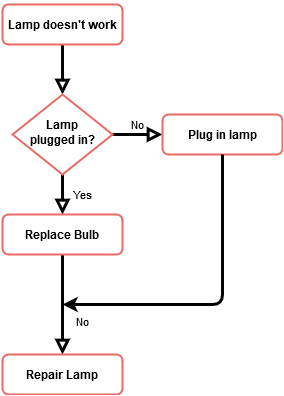
\includegraphics[height=6 cm, width=5cm]{images/Decision_control_3.png}
        	    % \caption{Caption}
        	    \label{fig:my_label}
        	\end{figure}
    \end{minipage}


\end{frame}

% \logo{
% 	\includegraphics[height=0.7cm]{images/logo_iai.jpg}
% 	\hspace{\dimexpr\paperwidth-2cm-5pt}
% 	\includegraphics[height=0.7cm]{images/logo_iai.jpg}
% 	}

\frame{\frametitle{Table of contents}
\tableofcontents\transdissolve
}
\AtBeginSection[]
  {
    \ifnum \value{framenumber}>1
      \begin{frame}<beamer>
      \frametitle{Plan}
      \tableofcontents[currentsection,currentsubsection]
      \end{frame}
    \else
    \fi
  }
% \AtBeginSection[currentsection, currentsubsection, hideothersubsection, sectionstyle=show/hide, subsectionstyle=show/shade] % Do nothing for \section*
% {\transblindshorizontal
% 	\begin{frame}<beamer>
% 		%\transdissolve
% 		\frametitle{currentsection}
% 		\tableofcontents[currentsection, hideothersubsections]%, pausesubsections]
% 	\end{frame}
% }

\section{Unit Outline}
    \begin{frame}{Unit-II Outline}
        \begin{itemize}
          
            \item Different syntax of if 
                \begin{itemize}
                        \item  Sequential execution of C program
                         \item if block
                            \item if else block
                            \item Nested if else block
                            \item if else-if else block
                \end{itemize}
       
            \item Logical Operators : AND ($\&\&$), OR ($||$) , NOT (!)
            \item ternary operators ( Expression ? a : b )
            \item comparison between if else and ternary operator
        \end{itemize}
    \end{frame}

\section{Different syntax of if }
    \begin{frame}{Sequential execution of program}
        \begin{minipage}{0.6 \textwidth}
                \lstinputlisting[language=C]{code/test-1.c}
        \end{minipage}%
         \begin{minipage}{0.4\textwidth}
                \begin{figure}
            	    \centering
            	    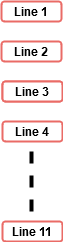
\includegraphics[height=5 cm, width=2 cm]{images/Sequential_execution.png}
            	    % \caption{Caption}
            	    %\label{fig:my_label}
        	\end{figure}
        \end{minipage}
    \end{frame}
    
    \subsection{if block}
        \begin{frame}{Basic syntax of \textbf{if block}}
                \begin{minipage}{0.3\textwidth}
                    \lstinputlisting[language=C]{code/basic-if-block-syntax.c}
                \end{minipage}%
                 \begin{minipage}{0.7\textwidth}
                    \begin{itemize}
                        \item The Expression is finally evaluated to binary value : \textcolor{green}{TRUE} or \textcolor{red}{FALSE}
                        \item Anything non-zero is treated as  \textcolor{green}{TRUE}
                    \end{itemize}      
                \end{minipage}
                        
            \begin{itemize}
                \item The statement 1 an statement 2 inside if block is executed only if Expression is evaluated to  \textcolor{green}{TRUE}
                \item In case if block contain only one statement, then the \{ \} after if(Expression) is optional.
            \end{itemize}
        \end{frame}
        
    \begin{frame}{C program using if block}
        \lstinputlisting[language=C]{code/cprogram-using-if-block.c}
        
    \end{frame}
    
     \begin{frame}{C program using if block with flow chart}
          \begin{minipage}{0.7\textwidth}
                \lstinputlisting[language=C]{code/cprogram-using-if-block.c}
            \end{minipage}%
            \begin{minipage}{0.3\textwidth}
                \begin{figure}
            	    \centering
            	    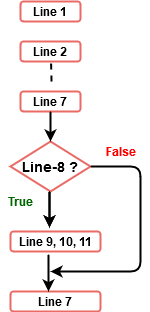
\includegraphics[height=6 cm, width=3 cm]{images/flow_chart-if-block.png}
            	    % \caption{Caption}
            
        	\end{figure}
        \end{minipage}
     \end{frame}
      
    \begin{frame}{Comparison symbol in C}
            \begin{figure}
            	    \centering
            	    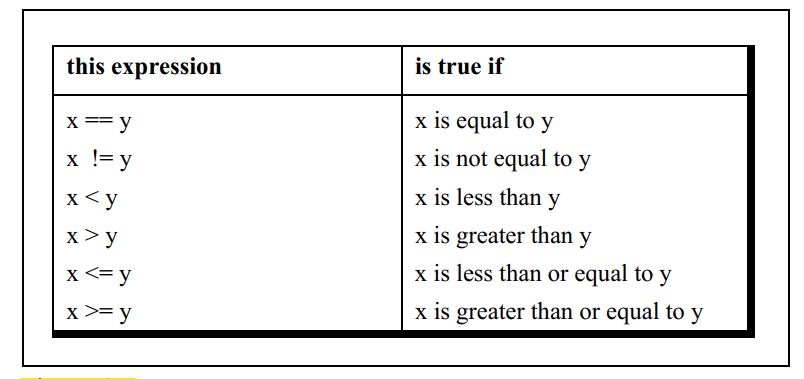
\includegraphics[height=5 cm, width=6 cm]{images/Logical_comparision_table.JPG}
            	   
        	\end{figure}
        
    \end{frame}
        
        
        

       \begin{frame}{C program examples for if block-2}
             \lstinputlisting[language=C]{code/if-prog-2.c}
        \end{frame}
    
 \subsection{if-else-block}
    \begin{frame}{Basic syntax of if-else block}
        \begin{minipage}{0.3 \linewidth}
            \lstinputlisting[language=C]{code/if-else-syntax.c}
        \end{minipage}%
        \begin{minipage}{0.7 \linewidth}
            \begin{figure}
            	    \centering
            	    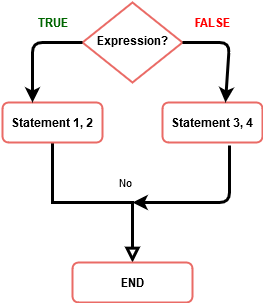
\includegraphics[height=5 cm, width=4 cm]{images/if-else-syntax.png}
            	    % \caption{Caption}
            	    %\label{fig:my_label}
        	\end{figure}
        \end{minipage}
        
        \begin{itemize}
            \item if the Expression value becomes \textcolor{green}{TRUE}, then the statement 1 ans statement 2 is executed.
            \item Otherwise statement 3 and statement 4 is executed.
        \end{itemize}    
        
    \end{frame}
    
    \begin{frame}{if else prog-1}
        \lstinputlisting[language=C]{code/if-else-prog-1.c}
    \end{frame}
    
    \begin{frame}{if-else prog-1 with flowchart}
        \begin{minipage}{0.7 \linewidth}
            \lstinputlisting[language=C]{code/if-else-prog-1.c}
        \end{minipage}%
        \begin{minipage}{0.3 \linewidth}
            \begin{figure}
            	    \centering
            	    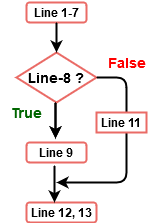
\includegraphics[height=5 cm, width=4 cm]{images/if-else-block-prg-1-flowchart.png}
            	    % \caption{Caption}
            	    %\label{fig:my_label}
        	\end{figure}
        \end{minipage}
        
    \end{frame}
    
    \begin{frame}{if-else program 2}
         \lstinputlisting[language=C]{code/if-else-prog-2.c}
    \end{frame}
\subsection{Exercise}
    \begin{frame}{Exercise if block}
        Let us C : Chapter 2
        \begin{itemize}
            \item[1.] Question A : a-e
            \item[2.] Question B : a-b
            \item[3.] Question C : a-b
            
        \end{itemize}
        
    \end{frame}
\end{document}
